\documentclass[runningheads]{llncs}

\usepackage[T1]{fontenc}
\usepackage{graphicx}
\usepackage{amsmath}
\usepackage{booktabs}
\usepackage{multirow}
\usepackage{siunitx}
\usepackage{array}
\usepackage{url}
\usepackage[hidelinks]{hyperref}

\sisetup{
  detect-all,
  round-mode=places,
  round-precision=3
}

\title{Explainability-Guided Distillation of Robust UAV Navigation Policies in a Noisy PyBullet Environment}
\titlerunning{Explainability-Guided Distillation for UAV Navigation}

\author{Anonymous Submission}
\authorrunning{Anonymous Submission}
\institute{Affiliation withheld for review}

\begin{document}
\maketitle

\begin{abstract}
We study whether a robust UAV navigation policy can also be recovered as a compact analytical controller. To do so, we build a custom Gymnasium-compatible environment on top of PyBullet and evaluate all reported models directly in the hardest stage-4 setting, which combines trajectory-aware rewards, noisy observations, Kalman-filtered state estimation, aerodynamic drag, wind gusts, and drifting obstacles. These perturbations are chosen to target specific failure modes rather than to act as generic randomization. We train SAC, TD3, DDPG, and PPO in this single-shot stage-4 environment and then analyze the learned controllers with decision-tree surrogates, LIME, SHAP, action-vector fields, Q-value landscapes, and rollout-aware equation fitting. The strongest result is that policy quality and policy distillability separate clearly: the final SHAP-guided SAC equation preserves 4/4 held-out stage-4 successes, whereas DDPG preserves 2/4 and TD3 preserves 0/4 under the same evaluation seeds. The recovered SAC law has the structure of a damped contextual potential field even though no such controller was hard-coded into the reward, and it avoids the local-minimum failures that trap an untuned artificial potential field on the same map. We therefore frame the paper as an empirical study of explainability-guided policy distillation for noisy continuous UAV navigation, rather than as a new RL method.
\keywords{UAV navigation \and reinforcement learning \and Kalman filtering \and explainable AI \and policy distillation}
\end{abstract}

\section{Introduction}
Learning-based UAV navigation is attractive because hand-crafted obstacle-avoidance rules often become brittle once sensing becomes noisy, obstacles drift, or dynamics deviate from the nominal model. At the same time, high-performing deep RL policies are difficult to audit, difficult to transfer, and difficult to compare beyond scalar reward. This raises a broader question: if a controller succeeds in a noisy environment, can its behavior be explained as a compact control law rather than only as a black-box network?

We address that question in a controlled simulation study. The environment is a custom Gymnasium-style task \cite{Brockman2016Gym} backed by PyBullet \cite{Coumans2021PyBullet}, with a 2D quadrotor-like agent navigating through mixed-shape obstacles toward a fixed goal. All experiments reported in the paper train directly in a single-shot stage-4 setting. That stage combines trajectory penalties, measurement noise, a Kalman filter \cite{Kalman1960}, aerodynamic drag, wind gusts, and obstacle drift. These perturbations are not arbitrary. They target the main failure modes seen in early policies: poor state estimation, overconfident straight-line motion, and sensitivity to mild distribution shift. In that sense, the environment behaves like a structured robustness benchmark inspired by sim-to-real randomization work \cite{Tobin2017DomainRandomization,Peng2018DynamicsRandomization}, but with perturbations that remain interpretable.

The second part of the paper focuses on explanation and distillation. We combine decision-tree surrogates, LIME \cite{Ribeiro2016LIME}, SHAP \cite{Lundberg2017SHAP}, vector-field plots, Q-value heatmaps, and rollout-aware equation extraction. The main empirical finding is that the best SAC controller behaves like a damped contextual potential field \cite{Khatib1986APF}: action depends primarily on raw goal displacement, velocity damping, and a short-range obstacle repulsion term. This structure was not hard-coded. It emerged from training and was recovered post hoc. By contrast, TD3 and DDPG can achieve strong task success while remaining much harder to summarize with the same interpretable controller family.

The contribution is therefore a combined environment-design, robustness, and explainability study with three concrete outcomes:
\begin{enumerate}
\item a staged noisy PyBullet environment for UAV navigation with a Kalman-filter state-estimation layer;
\item an explainability pipeline that goes beyond feature attribution and validates distilled equations in closed-loop rollouts;
\item empirical evidence that policy success and policy distillability are different properties, with SAC emerging as the most faithful analytical surrogate in our setting.
\end{enumerate}

\section{Related Work}
Deep RL has been used widely for navigation and obstacle avoidance in both ground and aerial robots, including continuous-control drone settings \cite{Marino2024KalmanRL,Huang2024QuadrotorSwarm}. However, much of that literature focuses on success rate and transfer robustness rather than on whether the learned policy can be turned back into a compact control law. Benchmarking work such as Arena-Bench \cite{Kastner2022ArenaBench} has also emphasized how sensitive obstacle-avoidance performance can be to environment dynamics and evaluation protocol. Our environment design follows that line of thought: we do not assume that clean-navigation success is enough to demonstrate robustness.

There is also a clear line of work on interpretable or explainable RL. Surveys by Milani et al.\ \cite{Milani2022XRL} and related explainable-robotics work \cite{Lee2023AdaptiveExplainable} show that explanation methods in RL range from saliency and attribution to symbolic surrogates, hierarchical skills, and policy extraction. SHAP \cite{Lundberg2017SHAP} and LIME \cite{Ribeiro2016LIME} have become standard post hoc explanation tools, while policy distillation \cite{Rusu2015PolicyDistillation} and verification-oriented extraction methods such as VIPER \cite{Bastani2018VIPER} aim to replace black-box policies with simpler surrogates. More recent work on concept-based policy distillation \cite{Bekkemoen2025ConceptDistill} further argues that interpretable latent concepts can preserve useful control structure.

Our work differs from those directions in two ways. First, the target is a continuous UAV-navigation controller, not a discrete toy domain or a concept-level explanation alone. Second, we treat \emph{closed-loop fidelity} as the key evaluation criterion for distillation. A surrogate with high one-step $R^2$ but poor rollout behavior is not considered faithful enough. This is the central methodological difference from many explanation pipelines, which stop at importance rankings or local linear explanations.

Finally, combining filtering and RL for navigation is itself not new. Marino and Guglieri \cite{Marino2024KalmanRL}, for example, combine an interacting multiple model Kalman filter with PPO for drone navigation. Our contribution is therefore narrower and, we believe, more defensible: in a custom PyBullet UAV environment, we combine a structured noise-and-dynamics benchmark, a Kalman-filter ablation, and rollout-validated analytical distillation. The novelty lies less in any single ingredient than in the way they are tied together to show a measurable gap between policy success and policy distillability.

\section{Environment and Training Setup}
\subsection{Custom Gymnasium/PyBullet Environment}
The environment is a 2D navigation task implemented with a Gymnasium interface \cite{Brockman2016Gym} and simulated in PyBullet \cite{Coumans2021PyBullet}. The UAV starts near one of four corners of a \SI{10}{m} square workspace and must reach a central goal while avoiding eight mixed-shape obstacles (spheres, cylinders, and boxes). The action is a 2D velocity command in $[-1,1]^2$ scaled by a maximum speed of \SI{15}{m/s}. The observation contains UAV position and velocity, goal displacement and distance, plus obstacle positions, radii, and shape codes.

Episodes run at \SI{240}{Hz} for up to \SI{18}{s}. Success occurs when the UAV reaches within \SI{0.65}{m} of the goal, or remains within \SI{1.0}{m} for 120 consecutive steps, without colliding. This definition prevents the agent from grazing the goal once and then drifting away.

\subsection{Stage-4 Robustness Setup}
All experiments in this paper use a single-shot stage-4 configuration. The reward combines a goal bonus, dense progress shaping, directional alignment, obstacle repulsion, a clearance bonus, a smoothness penalty, a near-miss penalty, a stall penalty, and a small per-step time cost. The state estimate is deliberately corrupted before it reaches the policy: position is perturbed by Gaussian noise with standard deviation \SI{0.05}{m}, velocity by \SI{0.10}{m/s}, the goal vector by \SI{0.05}{m}, and obstacle positions by \SI{0.08}{m}.

We then add dynamics and geometry perturbations that make memorized straight-line behavior brittle. The UAV is subjected to aerodynamic drag with coefficient $0.12$ and wind gust noise with standard deviation $0.35$. Obstacles drift around anchored nominal locations with per-step drift standard deviation $0.018$, damping $0.965$, and a maximum anchored offset of \SI{0.30}{m}. These perturbations are not generic domain randomization for its own sake. They are chosen to create the specific observation and dynamics mismatch that motivates filtering, robustness, and explainability in the single-shot stage-4 task.

\subsection{Kalman Filter}
In the stage-4 setup, the policy no longer sees the exact UAV state. Instead, the environment corrupts position and velocity with Gaussian noise and then fuses them through a Kalman filter:
\begin{align}
\hat{\mathbf{x}}_{t|t-1} &= \mathbf{F}\hat{\mathbf{x}}_{t-1|t-1}, \\
\mathbf{P}_{t|t-1} &= \mathbf{F}\mathbf{P}_{t-1|t-1}\mathbf{F}^\top + \mathbf{Q}, \\
\mathbf{K}_t &= \mathbf{P}_{t|t-1}\left(\mathbf{P}_{t|t-1} + \mathbf{R}\right)^{-1}, \\
\hat{\mathbf{x}}_{t|t} &= \hat{\mathbf{x}}_{t|t-1} + \mathbf{K}_t \left(\mathbf{z}_t - \hat{\mathbf{x}}_{t|t-1}\right),
\end{align}
where $\hat{\mathbf{x}} = [x, y, v_x, v_y]^\top$ and $\mathbf{F}$ is the constant-velocity transition matrix. In our implementation, the filter does not alter the physical state. It only improves the observation delivered to the policy. This distinction matters: the learned agent still has to act under noisy goals, drifting obstacles, drag, and wind, but it acts from a better state estimate.

\subsection{Training Protocol}
All policies discussed in the paper are trained directly in stage 4. SAC is represented by a single-shot stage-4 run with Kalman filtering enabled. TD3, DDPG, and PPO were tuned with Optuna and then trained sequentially for 5M steps each on the same stage-4 environment with 8 parallel environments. We also trained a matched stage-4 SAC run without the Kalman filter to isolate the effect of state estimation.

The explainability and distillation sections focus on the SAC controller that yielded the strongest and most stable analytical surrogate under stage-4 evaluation.

\section{Robustness Results}
\subsection{Algorithm Comparison}
Figure~\ref{fig:algo_compare} compares the smoothed evaluation success rate and reward curves for directly trained stage-4 SAC, TD3, DDPG, and PPO runs, clipped to the first \SI{1.05}{M} timesteps for readability. The single-shot stage-4 SAC run still reaches reliable success fastest and remains the strongest policy overall in this window. TD3 and DDPG both attain perfect evaluation checkpoints, but their curves are less stable and later regressions are visible outside the clipped window. PPO remains the weakest baseline in this environment, with a best recorded success rate of $62.5\%$.

\begin{figure*}[t]
\centering
\begin{minipage}[t]{0.49\textwidth}
\centering
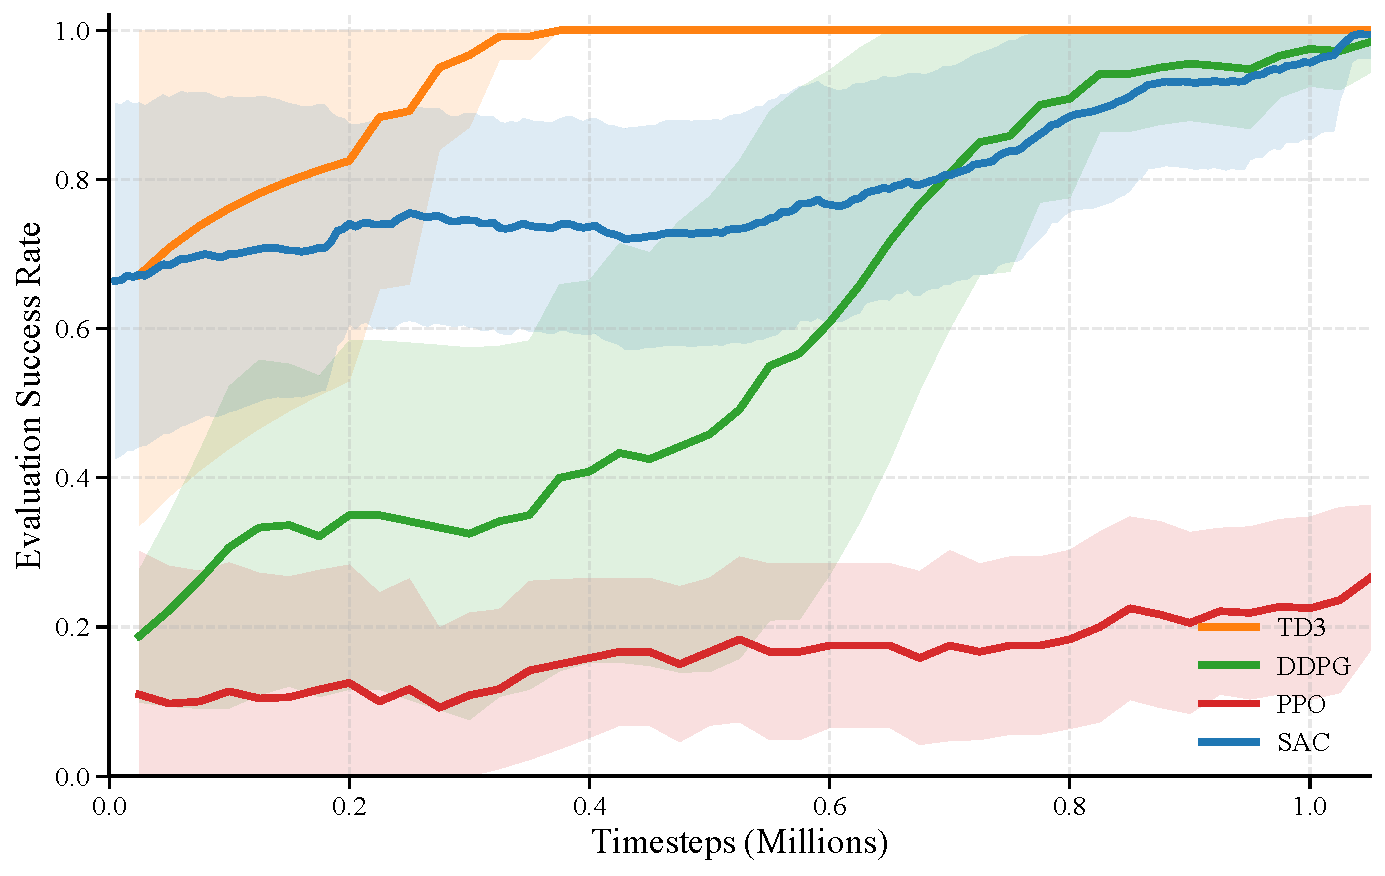
\includegraphics[width=\textwidth]{figures/paper_first_1050k_clean_success_rate.pdf}
\end{minipage}\hfill
\begin{minipage}[t]{0.49\textwidth}
\centering
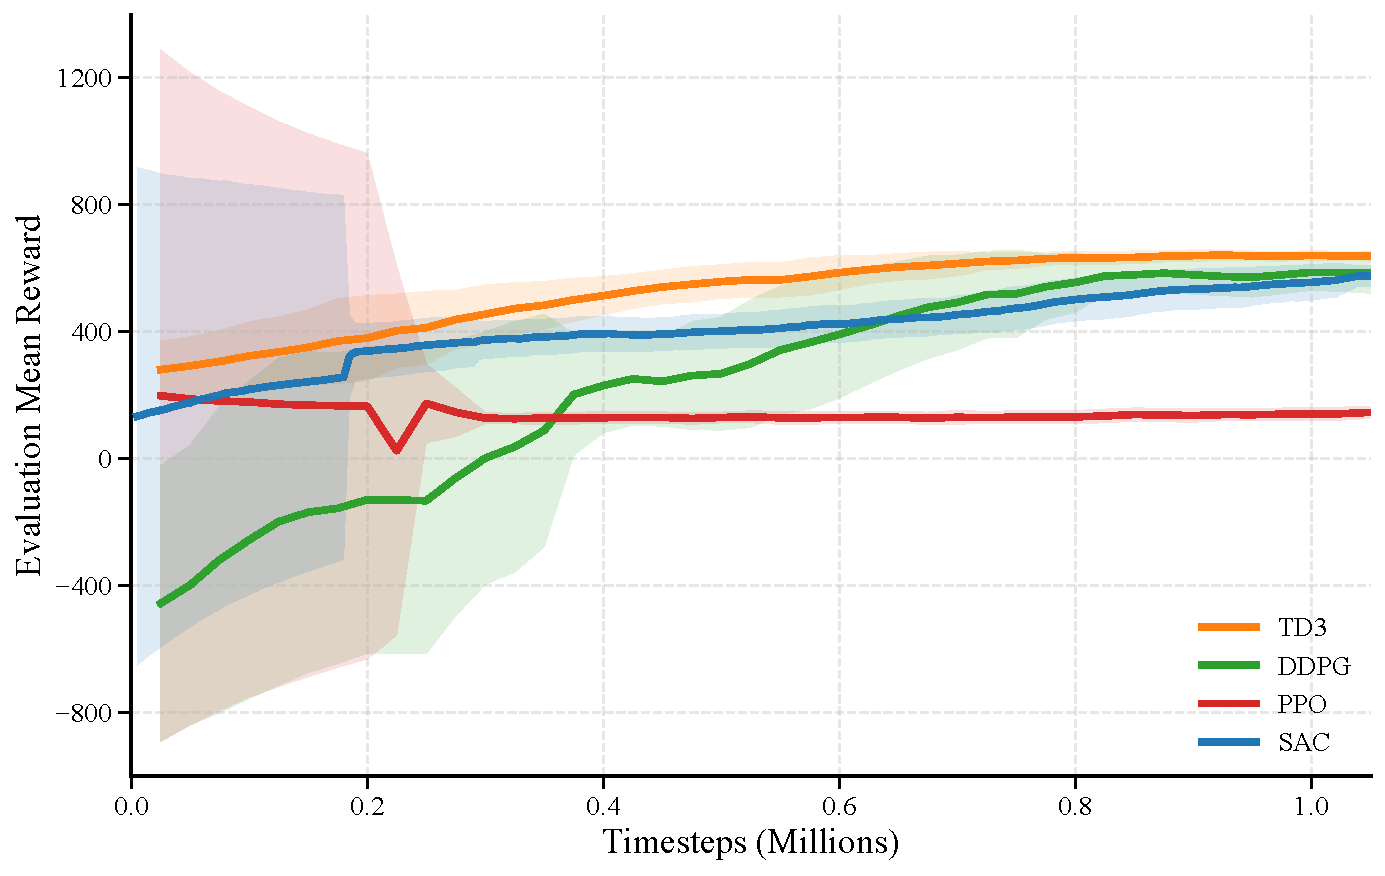
\includegraphics[width=\textwidth]{figures/paper_first_1050k_clean_mean_reward.pdf}
\end{minipage}
\caption{Evaluation success rate (left) and mean reward (right) for directly trained stage-4 SAC, TD3, DDPG, and PPO runs. The plots are clipped to the first \SI{1.05}{M} timesteps so that the early training dynamics can be compared on the same environment difficulty.}
\label{fig:algo_compare}
\end{figure*}

Table~\ref{tab:alg-summary} summarizes the strongest checkpoints and final distillation results. The important point is that high task success does not guarantee faithful distillation.

\begin{table}[t]
\caption{Summary of best policy checkpoints and final SHAP-equation fidelity at stage 4.}
\label{tab:alg-summary}
\centering
\footnotesize
\begin{tabular}{lccc}
\toprule
Policy & Best eval succ. & Eq. succ. & Trace dev. (m) \\
\midrule
SAC  & 1.000 & 1.000 & 2.154 \\
TD3  & 1.000 & 0.000 & 7.075 \\
DDPG & 1.000 & 0.500 & 3.557 \\
PPO  & 0.625 & --    & --    \\
\bottomrule
\end{tabular}
\end{table}

\subsection{Kalman Filter Ablation}
Figure~\ref{fig:kalman_ablation} shows stage-4 single-shot SAC training with and without the Kalman filter, clipped to the first \SI{1.05}{M} timesteps. The no-KF run can still reach successful checkpoints later in training, but it learns more slowly and is much more unstable. In our saved runs, the filtered single-shot SAC reached perfect evaluation success by \SI{1.65}{M} steps, while the no-KF variant required \SI{6.3}{M} steps to reach its best perfect checkpoint and later collapsed to zero success in its final evaluation.

\begin{figure*}[t]
\centering
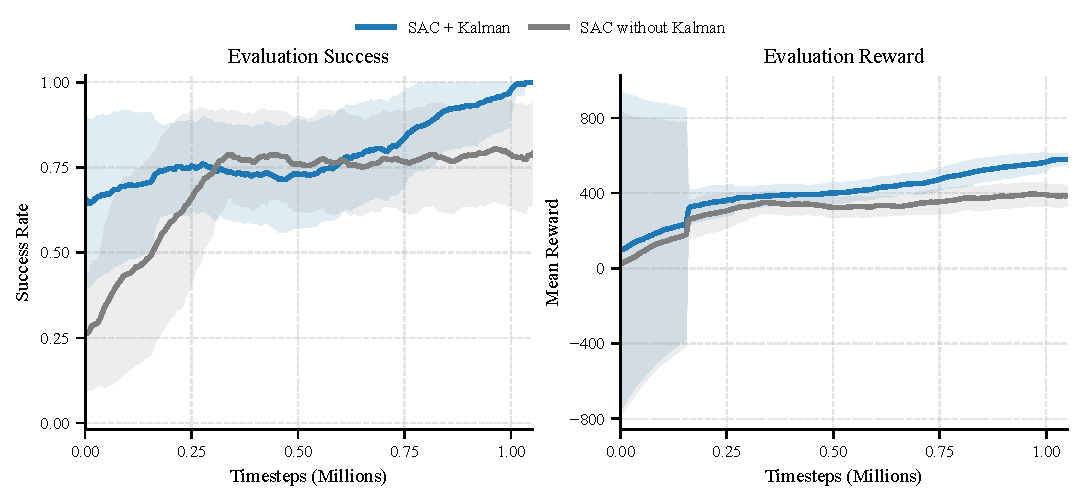
\includegraphics[width=\textwidth]{figures/kalman_ablation.pdf}
\caption{Stage-4 single-shot SAC with and without the Kalman filter. The filter improves learning speed and stabilizes training by reducing the variance of the state estimate seen by the policy.}
\label{fig:kalman_ablation}
\end{figure*}

The practical role of the filter is simple: it converts noisy position/velocity measurements into a smoother latent state before the policy maps observation to action. In our environment, that reduces spurious velocity corrections and makes the policy less brittle to the added drag, wind, and obstacle drift.

\section{Explaining the Learned Policy}
\subsection{Potential-Field-Like Behavior}
Figure~\ref{fig:interp_panel} shows the core qualitative evidence that the main SAC policy learned a control strategy reminiscent of an artificial potential field \cite{Khatib1986APF} even though such a field was not explicitly coded into the reward. The action-vector field is plotted only over free space, so the arrows indicate how the controller bends around obstacles rather than cutting through them. The Q-value landscape forms a smooth basin around safe goal-reaching trajectories. Most importantly, the potential-field comparison now makes the failure mode explicit: an untuned APF creates a non-goal local minimum that traps the trajectory, whereas the trained stage-4 SAC policy escapes the same region and reaches the goal.

\begin{figure*}[t]
\centering
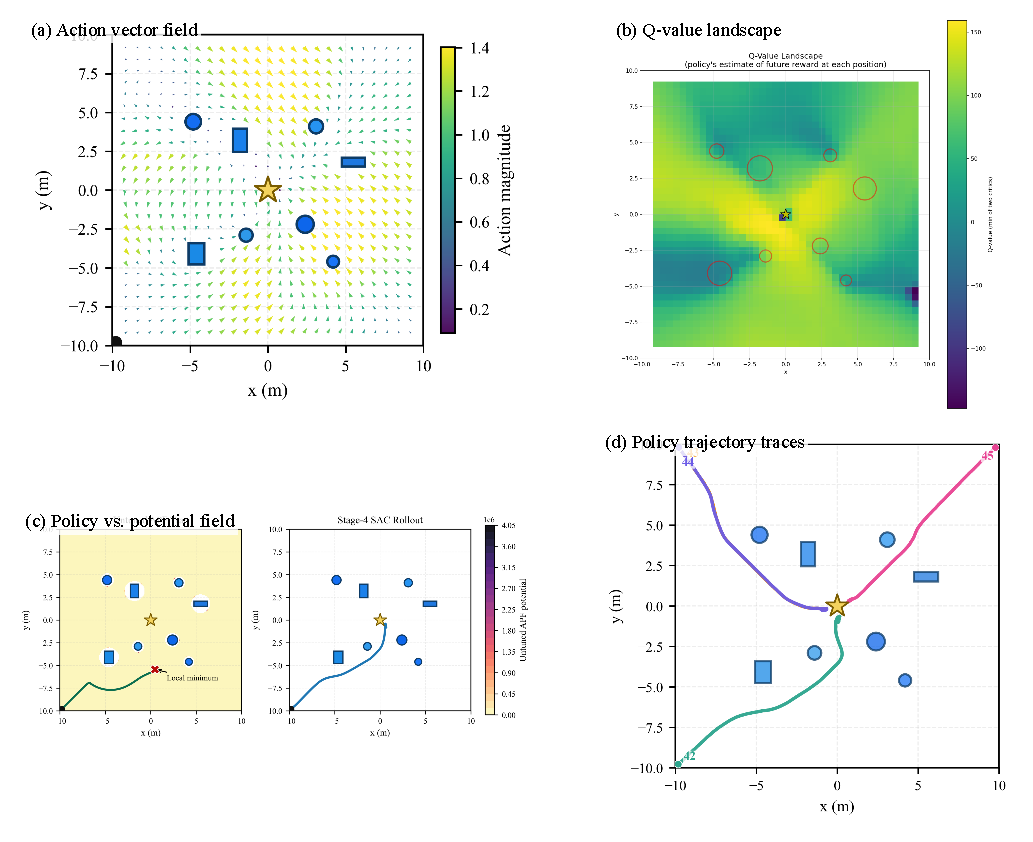
\includegraphics[width=\textwidth]{figures/interpretability_panel.pdf}
\caption{Qualitative interpretation of the main SAC policy. (a) Action-vector field induced by the learned actor, plotted only in free space so obstacle interiors do not visually imply invalid actions. (b) Q-value landscape showing a smooth high-value basin near safe goal-reaching trajectories. (c) Untuned artificial potential field: the left panel shows a local-minimum trap, while the right panel shows the trained stage-4 SAC policy reaching the goal from the same start. (d) Representative trajectory traces. Together these plots suggest that the policy learned a potential-well-like structure without inheriting the classical local-minimum failure of a naive potential field.}
\label{fig:interp_panel}
\end{figure*}

\subsection{Decision Trees, LIME, and SHAP}
We used three complementary post hoc explanation tools. A shallow decision-tree regressor provides discrete if/then rules; LIME gives local linear explanations around selected states; and SHAP supplies global feature-attribution summaries. For the main SAC policy, the decision-tree fit reached $R^2 = 0.826$ for the $x$-action and $R^2 = 0.670$ for the $y$-action. The learned rules split primarily on raw goal displacement for action $x$ and on goal displacement together with repulsion for action $y$. That is already suggestive: the tree rediscovers a goal-seeking controller with directional obstacle corrections.

The SHAP and LIME panels in Fig.~\ref{fig:xai_panel} make the same pattern more explicit. Goal displacement and the UAV state dominate attribution, while individual obstacle coordinates have lower global importance. However, a purely goal-directed explanation is insufficient in closed loop. Obstacle-aware terms are needed to preserve safe behavior, especially in the final stage-4 evaluation. This is one reason why we do not stop at SHAP plots alone.

\begin{figure*}[t]
\centering
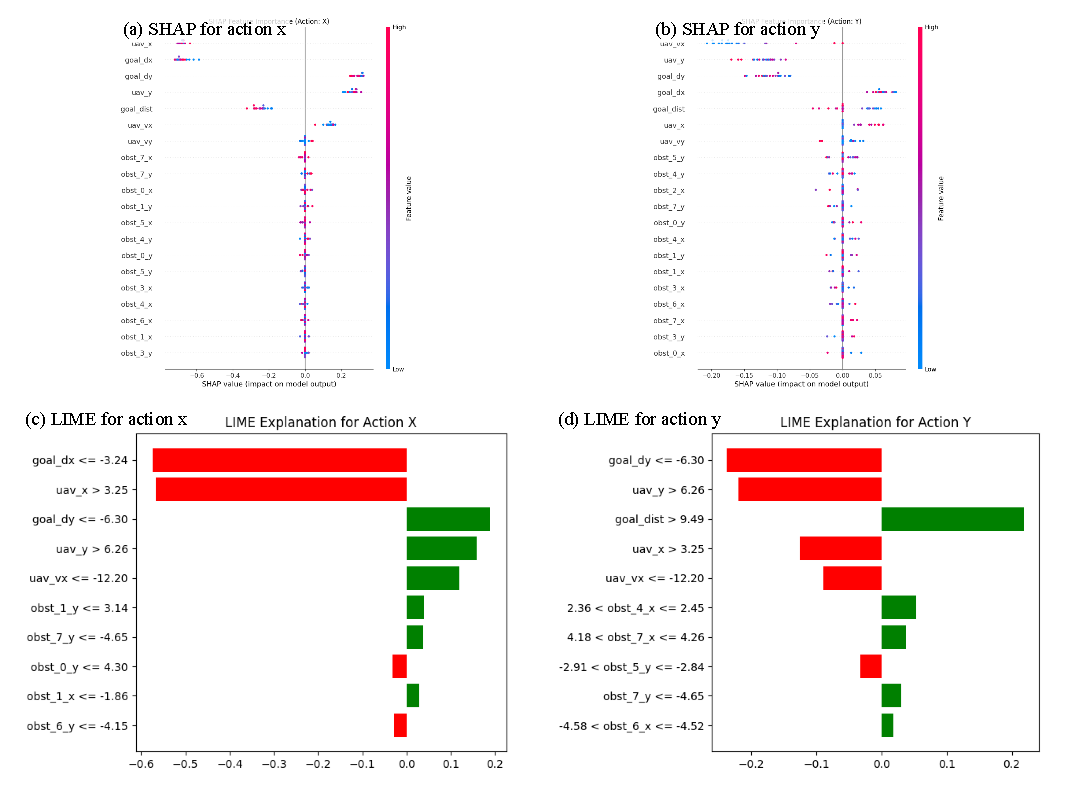
\includegraphics[width=\textwidth]{figures/explainability_panel.pdf}
\caption{Post hoc explanations for the main SAC policy. SHAP gives global feature-importance summaries for both action dimensions, while LIME highlights local directional explanations around a representative state. Goal displacement and velocity dominate globally, but local obstacle-aware corrections remain necessary for faithful closed-loop behavior.}
\label{fig:xai_panel}
\end{figure*}

\subsection{Rollout-Aware Equation Distillation}
Based on these explanations, we fit a family of compact analytical controllers using raw goal displacement, velocity damping, and short-range obstacle repulsion terms. Importantly, we select the final equation by held-out rollout success first, then trace deviation, and only then by one-step $R^2$. This avoids the common failure mode where a surrogate looks excellent on sampled states but diverges quickly in closed loop.

The final SAC equation selected at stage 4 is
\begin{align}
a_x &= 0.0427 + 0.1442\,\texttt{goal\_dx} - 0.0120\,v_x + 0.4725\,r_x, \\
a_y &= -0.0624 + 0.1144\,\texttt{goal\_dy} - 0.0071\,v_y + 0.6592\,r_y,
\end{align}
where $(r_x, r_y)$ denotes a nearest-obstacle repulsion vector with exponential decay inside a \SI{4.5}{m} threshold. On held-out validation rollouts, this equation preserved 4/4 successes and achieved a mean trajectory deviation of \SI{2.154}{m}. The result is important because the same extraction pipeline does \emph{not} work equally well for all successful policies: DDPG preserves only 2/4 successes and TD3 preserves 0/4 under the same stage-4 seeds.

\section{Trajectory-Level Distillation Results}
Figure~\ref{fig:stage4_traj} compares the original policies against their final stage-4 SHAP-guided equations. SAC is the clearest success case. Its analytical surrogate tracks the original policy closely enough to preserve all evaluated successes. DDPG is partially distillable but still inconsistent across seeds. TD3 has excellent one-step regression in some settings, yet its rollout behavior diverges badly; it is therefore an example of why closed-loop validation matters.

\begin{figure*}[t]
\centering
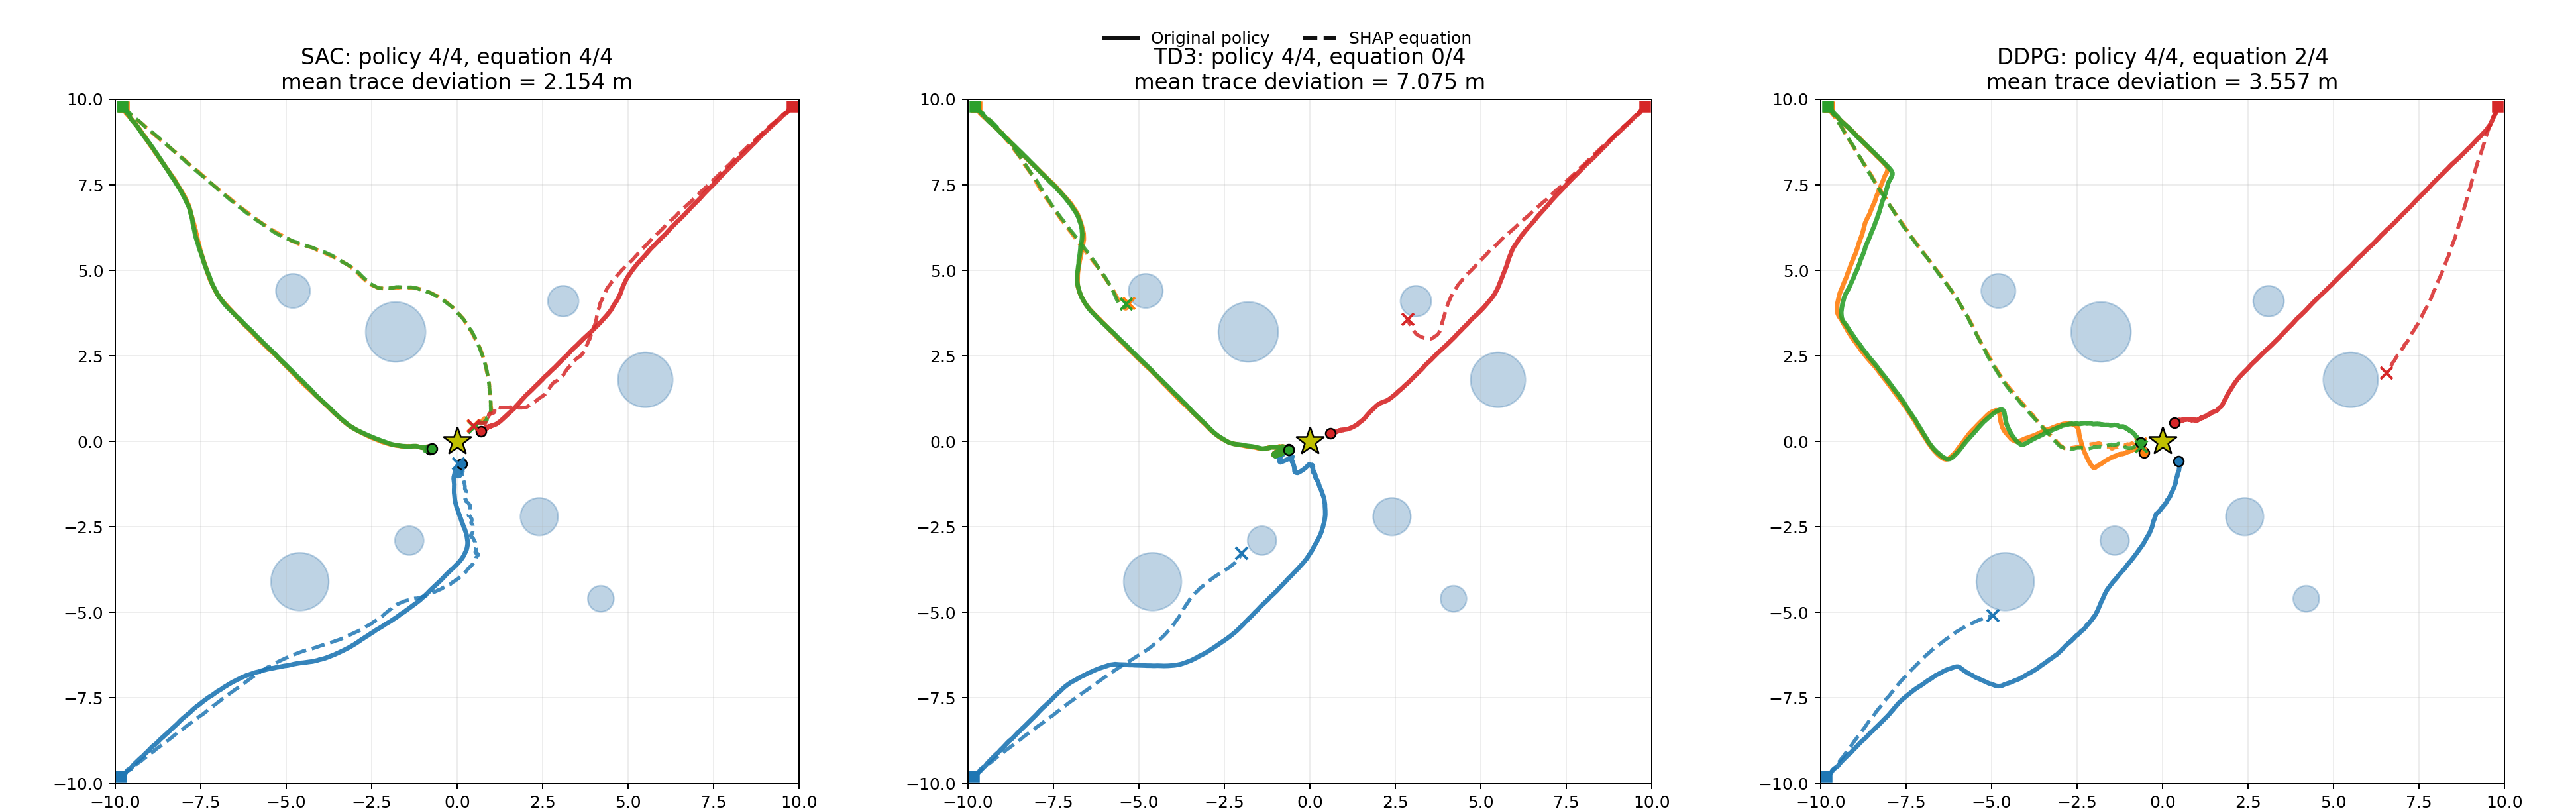
\includegraphics[width=\textwidth]{figures/stage4_shap_trajectories.png}
\caption{Stage-4 trajectory overlays for the original policies and their final rollout-selected SHAP equations. SAC remains the strongest case: the distilled analytical controller preserves all four held-out successes. DDPG is partially faithful, while TD3 diverges in closed loop despite successful original rollouts.}
\label{fig:stage4_traj}
\end{figure*}

This gap between task success and distillability is the main empirical message of the paper. A policy can solve the task while still being hard to summarize as a compact control law. In our experiments, SAC appears to learn a smoother and more structured controller than TD3 or DDPG in the same noisy environment.

\section{Discussion and Limitations}
The most important lesson from these experiments is that robustness and interpretability are related but not identical objectives. Stage-4 SAC, TD3, and DDPG can all reach perfect evaluation checkpoints, yet only SAC consistently admits a compact analytical surrogate with acceptable closed-loop fidelity. In other words, solving the task is not enough; some policies remain far easier to compress into a control law than others.

That observation also clarifies the scope of the paper. We are not proposing a new RL algorithm, nor are we claiming the first use of Kalman filtering, SHAP, or LIME in navigation. The contribution is the synthesis: a structured noisy benchmark, a controlled state-estimation ablation, and a trajectory-level distillation pipeline that tests whether an interpretable surrogate can actually fly the task. Within that setup, SAC is the clearest positive case and TD3 is the clearest counterexample.

The work nevertheless has important limitations. The environment is custom and two-dimensional, so the conclusions are strongest as a case study rather than as a universal statement about all UAV controllers. The explanation pipeline is still post hoc: it reveals meaningful structure in the learned controller, but it does not guarantee causal sufficiency or formal interpretability. In addition, although the algorithm-comparison plots now use matched stage-4 single-shot runs, the deeper interpretability case study still centers on the SAC controller that produced the most faithful analytical surrogate.

Despite those limitations, the evidence supports one strong conclusion: if the goal is not only to learn a high-performing policy but also to recover a compact analytical surrogate, SAC is the most promising controller family among the methods tested here.

\section{Conclusion}
We introduced a custom Gymnasium/PyBullet UAV-navigation environment and evaluated all reported policies in a single-shot stage-4 setting that combines noisy observations, Kalman-filtered state estimation, drag, wind, and drifting obstacles. We then analyzed the learned policies with decision trees, LIME, SHAP, vector fields, Q-value heatmaps, and trajectory-level distillation.

The central finding is that SAC is not just the best-performing policy in our experiments; it is also the most \emph{distillable}. Its final SHAP-guided equation preserves stage-4 rollout success and exposes a compact damped potential-field-like controller that was never hard-coded. This suggests a useful research direction for future work: evaluating learned policies not only by reward and success rate, but also by the fidelity of the simplest analytical controller that can reproduce them.

\bibliographystyle{splncs04}
\bibliography{references}

\end{document}
